\documentclass[10pt]{article}

% set smaller margins
\usepackage[a4paper,margin=1in]{geometry}

% use standard math symbols
\usepackage{amssymb}

% for \text inside formulas and for \eqref
\usepackage{amsmath}

% for bibliography
\usepackage{natbib}
\bibliographystyle{plainnat}

% enable full XeLaTeX power
\usepackage{xltxtra}

% select widely available fonts
\setmainfont{Georgia}
\setmonofont{Courier New}

% substitute another font for a few Unicode glyphs missing in the main font
\newfontfamily{\msminchofont}{MS Mincho}
\catcode`✓=\active
\protected\def ✓{{\msminchofont\char`\✓}}

% set paragraph margins
\setlength{\parindent}{0pt}
\setlength{\parskip}{6pt plus 2pt minus 1pt}

% prevent overfull lines
\setlength{\emergencystretch}{3em}

% for \includegraphics
\usepackage{graphicx}
\usepackage{grffile}

% fit images in page width
\makeatletter
\def\maxwidth{\ifdim\Gin@nat@width>\linewidth\linewidth
\else\Gin@nat@width\fi}
\makeatother
\let\Oldincludegraphics\includegraphics
\renewcommand{\includegraphics}[1]{\Oldincludegraphics[width=\maxwidth]{#1}}

% for exact placement of figures
\usepackage{float}

% for footnotes in tables
\usepackage{longtable}
\usepackage{booktabs}

% for hyperlinks
\usepackage[colorlinks,urlcolor=blue,filecolor=blue,linkcolor=black,citecolor=black]{hyperref}
\usepackage[all]{hypcap}
\urlstyle{same}

% do not number sections
\setcounter{secnumdepth}{0}


% remove date completely
\date{\vspace{-5ex}}

\begin{document}


\subsection{Deep Reinforcement Learning Based Control in Continuous
Action and State Spaces using Policy Gradients and Actor-Critic
Networks}

\subsubsection{Experiments}

\textbf{Cart Pole with Discrete Action}

The cart-pole model(2) has four state variables

\[
x - \text{position of the cart on the track} \\
\theta - \text{angle of the pole with the vertical} \\
\bar{x} - \text{cart velocity} \\
\bar{\theta} - \text{rate of change of the angle}
\]

\begin{itemize}
\item
  Observation 1:* Comparing Fig 1 and Fig 2, it is clear that having a
  larger batch size helps in faster learning and better policies in
  terms of Average Returns.
\item
  \emph{Observation 2:}** **From Fig 3 it is clear that when we push up
  the probability of picking action at in state st in proportion to the
  ‘reward-to-go’ from that state-action pair—the sum of rewards achieved
  by starting in st, taking action at, and then acting according to the
  current policy forever after, rather than a trajectory centric policy
  gives much better policies.
\end{itemize}

Also Advantage normalization gives slightly better policies.

\begin{itemize}
\item
  Observation 3: However having a baseline didn’t improve the policy as
  expected as shown in figure 3.
\end{itemize}

\begin{figure}
\centering
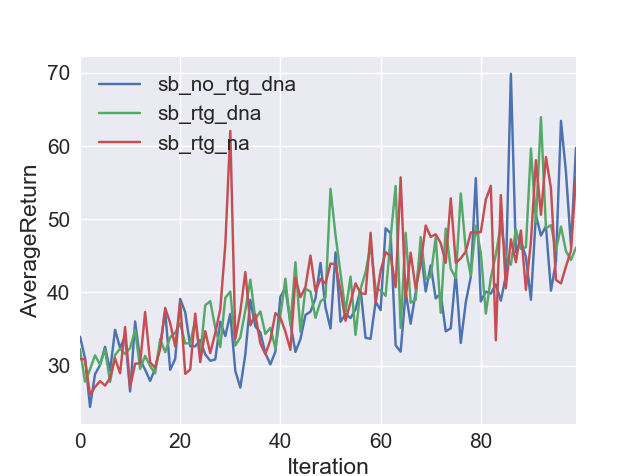
\includegraphics{Images/graph_small_batch.png}
\caption{}
\end{figure}

Figure 1

\begin{figure}
\centering
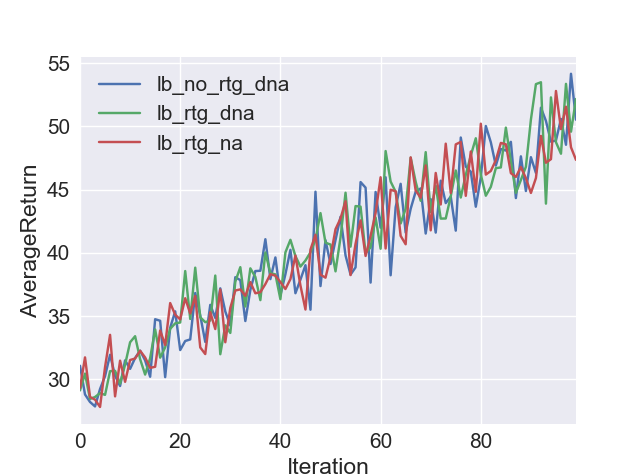
\includegraphics{Images/graph_large_batch.png}
\caption{}
\end{figure}

Figure 2

\begin{figure}
\centering
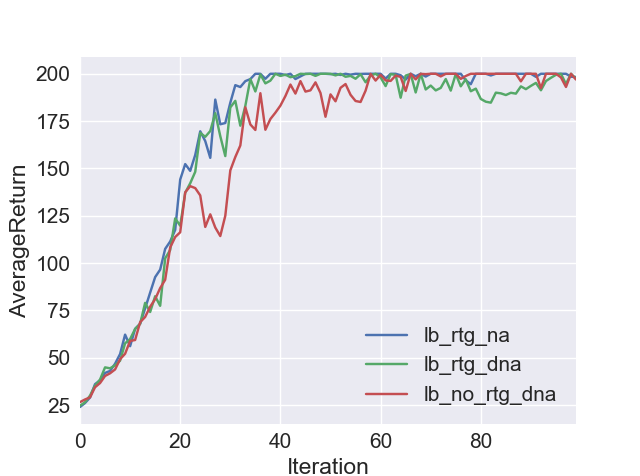
\includegraphics{Images/large_optimal.png}
\caption{}
\end{figure}

Figure 3

\begin{figure}
\centering
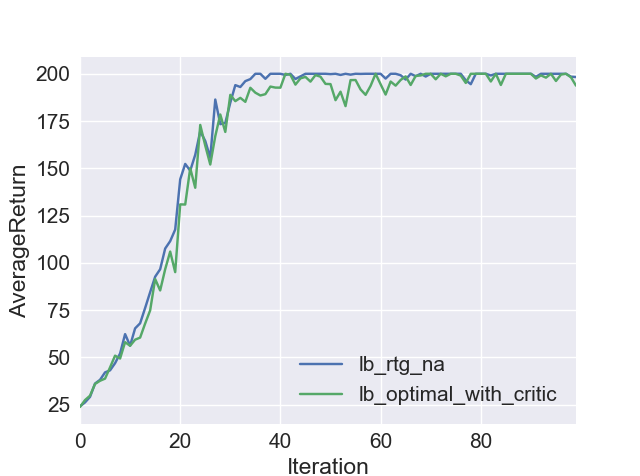
\includegraphics{Images/with-without-critic.png}
\caption{}
\end{figure}

Figure 4

\textbf{Inverted Pendulum with Continuous Actions}

\begin{figure}
\centering
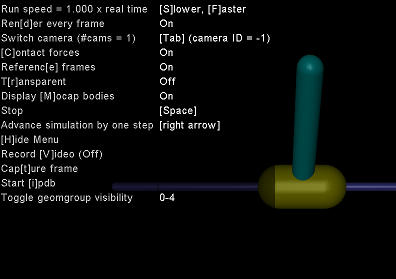
\includegraphics{Images/pendulum_continuous.PNG}
\caption{}
\end{figure}

Figure 5

\begin{itemize}
\item
  Observation 1: The learning curves with two different network
  architectures is shown in Fig 6. Its clear from the graph that the 5
  layered feed forward neural network learned better policies in lesser
  number of iterations.
\end{itemize}

Command Line Code

\begin{verbatim}
python train_pg.py InvertedPendulum-v2 --render -n 100 -b 5000 -e 5 -rtg --exp_name lb_continuous_5_layered_DeepNeuralNet -l 3 -lr 1e-2
\end{verbatim}

\begin{figure}
\centering
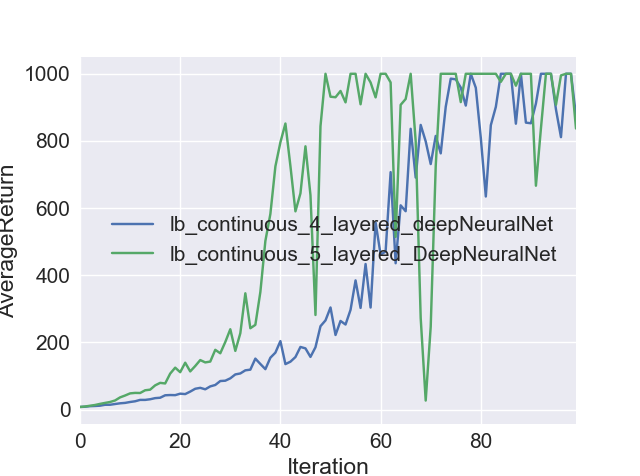
\includegraphics{Images/inverted.png}
\caption{}
\end{figure}

Figure 6

\textbf{HALF CHEETAH}

Half-Cheetah(1), is a planar kinematic string of 9 links and 10 joints;
the “paws” of Half-Cheetah will also be called joints. The angles of
4-th and 5-th joint are fixed, all the the others are controllable.
Consequently, Half-Cheetah is a 6-degree-of-freedom walking robot.

\begin{figure}
\centering
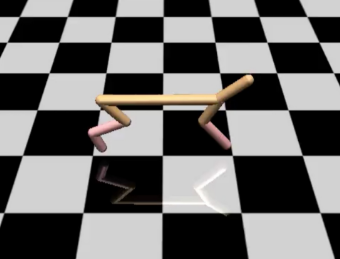
\includegraphics{Images/half-ch.PNG}
\caption{}
\end{figure}

Figure 7

\begin{figure}
\centering
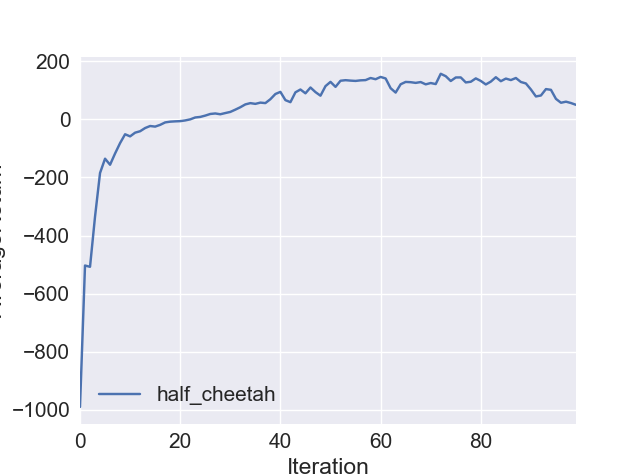
\includegraphics{Images/half-cheetah.png}
\caption{}
\end{figure}

Figure 8

Code Block

\begin{verbatim}
python train_pg.py HalfCheetah-v2 -ep 150 --discount 0.9 -b 40000 -rtg -l 3 -s 32 -lr 4e-2 --exp_name half_cheetah
\end{verbatim}

\emph{Observation 1:} After a lot of hyper parameter tuning, the
settings that gave an average return above 150 before 100 iterations is
given in the code block below. It used an unusually high batch size and
a 5 layered deep neural network without a critic. * *

\subsubsection{REFERENCES}

\begin{enumerate}
\def\labelenumi{\arabic{enumi}.}
\item
  Learning to Control a 6-Degree-of-Freedom Walking Robot Paweł
  Wawrzynski,
\end{enumerate}

http://prac.elka.pw.edu.pl/\textasciitilde{}pwawrzyn/pub-s/0601\_SLEAC.pdf

\begin{enumerate}
\def\labelenumi{\arabic{enumi}.}
\item
  A. G. Barto, R. S. Sutton, and C. W. Anderson, “Neuronlike adaptive
  elements that can solve difficult learning control problems,”
  http://www.derongliu.org/adp/adp-cdrom/Barto1983.pdf
\end{enumerate}


\end{document}
